\newpage
\chapter{Pruebas de Funcionalidad}
\section{Aspectos Generales}
Una prueba funcional es una prueba basada en la ejecución, revisión y retroalimentación de las funcionalidades previamente especificadas para un software. Realizada para encontrar errores o defectos en la implementación o diseño del mismo.\\
El diseño del plan de pruebas de funcionalidad, debe partir de la especificación explicita de las pruebas. Los objetivos específicos de las pruebas deben enunciarse en términos medibles. Por ejemplo: la efectividad de las pruebas, su cobertura, el tiempo medio antes de aparecer una falla, el costo por descubrir y corregir defectos, la frecuencia de ocurrencia, las horas de trabajo de pruebas.\\Además, conviene realizar las pruebas usando perfiles y usuarios reales del software, esto con el fin de tener el escenario más real posible para pruebas.
\section{Estrategias de Prueba para Software Convencional}
\subsection{Pruebas de Unidad}
\paragraph{Verifican el código escrito.} 
Son pruebas que se enfocan en cada componente de manera individual, lo que garantiza que funcionan adecuadamente como unidad. Estas pruebas utilizan mucho de las técnicas de prueba que ejercitan rutas especificas en una estructura de control de componentes para asegurar una cobertura completa y la máxima detección de errores.\\
Las pruebas de unidad enfocan los esfuerzos de verificación en la unidad más pequeña del diseño de software: el componente o módulo de software. Se usan las descripciones de diseño del componente (un ejemplo de esta descripción, es la descripción de casos de uso que se realiza comúnmente en el diseño de software) como guía, para establecer las rutas de control más importantes, las cuales se prueban para descubrir errores dentro del módulo.\\ Las pruebas de unidad se enfocan en la lógica de procesamiento interno y de las estructuras de datos dentro de las fronteras de un componente. Estas pruebas pueden realizarse en paralelo para múltiples componentes.\\
\subsubsection{Consideraciones}
\begin{enumerate}
	\item La interfaz del módulo se prueba para garantizar que la información fluya de manera adecuada hacia y desde la unidad de software que se esta probando. Es la primer prueba que se debe hacer, ya que si los datos no entran o salen de manera adecuada, todas las demás pruebas resultan irrelevantes.
	\item Las estructuras de datos locales se examinan para asegurar que los datos almacenados temporalmente mantienen su integridad durante todos los pasos en la ejecución de un algoritmo o rutina.
	\item Todos los posibles flujos dentro de un módulo deben de ser ejecutados al menos una vez. Los casos de prueba deben de diseñarse para describir errores debidos a cálculos erróneos, comparaciones incorrectas o flujos de control inadecuados.
	\item Se deben establecer condiciones de frontera que especifiquen los limites de funcionalidad y procesamiento que cada unidad tiene.  Además de que en estas pruebas deben ser considerados los casos en que las estructuras de datos y de control sean evaluados en sus valores mínimos, máximos y con valores por debajo y por encima de estos respectivamente, ya que comúnmente es en estas situaciones cuando se detectan fallos dentro del software.
	\item Se deben poner a prueba todas las rutas para el manejo de errores. Estas rutas deben de haber sido consideradas si se aplico un buen diseño, ya que estos anticipan los errores y establecen las ya mencionadas rutas.
\end{enumerate}
\subsubsection{Procedimiento}
Las pruebas de unidad por lo general se realizan al mismo tiempo que la codificación. El diseño de las pruebas de unidad puede ocurrir antes de comenzar la codificación o después de haber generado el código. La especificación de requerimientos y el diseño posterior, proveen la información necesaria para establecer los casos de prueba. Cada caso de prueba debe acoplarse con un conjunto de resultados esperados.\\
Dado que un componente no es un programa independiente, con frecuencia debe desarrollarse un software especial que apoye en esta tarea (comúnmente denominado como software controlador). En la mayoría de los casos, un controlador, no es más que un <<programa principal>> que acepta datos de caso de prueba, paso estos datos al componente (que se probará) y muestra los resultados obtenidos.\\ En caso de que el módulo invoque a otros módulos durante su ejecución, es necesario el uso de <<representantes>> (o stubs en inglés) los cuales sirven para sustituir módulos que estén subordinados al componente que se va a probar.\\
Los controladores y representantes es un extra que se debe realizar en las pruebas, ya que no son entregados en el producto final. En caso de que el componente de software utilice para su ejecución de muchos otros componentes y la generación de controladores y representantes resulte muy costosa. Es posible posponer las pruebas de ese módulo hasta las pruebas de integración. Mientras más simple sea el módulo, más sencillo resultara probarlo.
\subsection{Pruebas de Integración}
\paragraph{Verifican el diseño del software.}
Posteriormente a las pruebas de integración, los componentes deben de ensamblarse o integrarse para formar un paquete de software completo. La prueba de integración aborda los conflictos asociados con los problemas duales de verificación y construcción de programas.\\ Durante la integración, se usan más las técnicas diseño de casos de prueba que se enfocan en entradas y salidas, aunque también pueden usarse técnicas que prueben rutas de programa especificas para asegurar la cobertura de las principales rutas de control.\\ Las pruebas de de integración son una técnica sistemática para construir la arquitectura del software mientras se llevan a cabo pruebas para descubrir errores asociados a la interfaz. El objetivo es tomar los componentes probados de manera individual y construir la estructura de programa especificada en el diseño.\\ Comúnmente la integración no es hecha de manera incremental, lo cual puede generar diversos problemas, ya que el programa es probado como un todo, todos los componentes son combinados por adelantado. Con esto, la corrección de errores se dificulta pues el aislamiento de las causas se complica por la vasta extensión de todo el programa.\\
La integración incremental es lo contrario al enfoque anterior, pues el software se construye y prueba en incrementos pequeños, donde los errores sean más fáciles de aislar y corregir, las interfaces tienen más posibilidades de probarse por completo y puede aplicarse un enfoque de prueba sistemático.
\subsubsection{Integración descendente}
La prueba de integración descendente es un enfoque incremental a la construcción de la arquitectura de software. Los módulos se integran al moverse hacia abajo a través de la jerarquía de control, comenzando por el módulo de control principal, los módulos que dependan de este se incorporan en la estructura en una forma de primero profundidad o primero en anchura.\\ La integración primero en profundidad integra todos los componentes sobre una ruta de control mayor de la estructura del programa. La selección de la ruta mayor resulta arbitraria y depende de las características de la aplicación.
En la figura 2.1 se puede apreciar su funcionamiento, considerando que la primera integración a realizarse sería la de M1-M2-M5-M8 (siendo cada uno de estos la representación gráfica de un módulo).
\begin{figure}[H]
	\centering
	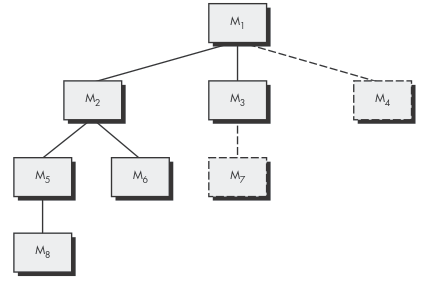
\includegraphics[scale=1]{project/images/profundidad.png}
	\caption{\textbf{Integración descendente}}
\end{figure}
Posteriormente se integrara M6, y finalmente se construyen las rutas de control central (M1-M3-M7) y derecha (M1-M4).\\
La integración primero en anchura incorpora todos los componentes directamente subordinados en cada nivel y se mueve horizontalmente a través de la estructura.\\ Continuando con el ejemplo anterior, los componentes M2-M3-M4 se probarían primero. Después en el siguiente nivel de control M5-M6.
En general, el proceso de integración se realiza en una serie de 5 pasos:
\begin{enumerate}
	\item El módulo de control principal se usa como un controlador de prueba y los representantes (stubs) se sustituyen con todos los componentes directamente subordinados (que son invocados) al módulo de control principal.
	\item Dependiendo del enfoque de integración seleccionado (primero profundidad o primero anchura), los representantes subordinados se sustituyen uno a la vez con componentes reales.
	\item Las pruebas se llevan a cabo conforme se integra cada componente.
	\item Al completar cada conjunto de pruebas, otro representante se sustituye por el componente real.
	\item Las pruebas de regresión pueden realizarse para asegurar que no se introdujeron nuevos errores.
\end{enumerate}
Este proceso se repite desde el paso 2 hasta que se construye toda la estructura del programa.\\
La estrategia de integración descendente verifica los principales puntos de control al principio de cada proceso de prueba. Si se selecciona la integración primero en profundidad, es posible implementar y demostrar el funcionamiento completo del sistema. La integración descendente tiene como complicaciones cuando es necesario que ocurra un procesamiento en los niveles bajos de la jerarquía a fin de probar de manera adecuada los niveles superiores. Ya que al principio de las pruebas, los representantes sustituyen a los módulos de bajo nivel, por lo tanto ningún dato significativo puede fluir hacia arriba en la estructura del programa.\\
Una alternativa para evitar esta problemática resulta en evaluar primero a los módulos con menor jerarquía y posteriormente a los de mayor, a esta estrategia se le conoce como estrategia de integración descendente.\\
\subsubsection{Integración ascendente}
Esta estrategia comienza con la construcción y prueba de módulos atómicos (componentes en los niveles inferiores de la estructura del programa). Puesto que los componentes se integran de abajo hacia arriba, la funcionalidad que proporcionan los componentes subordinados en determinado nivel siempre esta disponible y se elimina la necesidad de representantes.\\
Una estrategia de integración ascendente puede implementarse con los siguientes pasos:
\begin{enumerate}
	\item Los componentes en el nivel inferior se combinan en grupos (llamados construcciones o <<builds>>) que realizan una subfunción de software especifica.
	\item Se escribe un controlador a fin de coordinar la entrada y salida de casos de prueba.
	\item Se prueba el grupo.
	\item Los controladores se remueven y los grupos se combinan moviéndolos hacia arriba en la estructura de programa.
\end{enumerate}
En la figura 2.2 se ejemplifica la integración ascendente. A los módulos de baja jerarquía se les agrupa, en el ejemplo se formaron tres grupos, los cuales están relacionados directamente con un controlador el cual coordinara las entradas y salidas de estos. Los controladores son representados con la letra <<D>> y su respectivo subíndice.\\
Posterior a la realización de las pruebas, los controladores son remplazados por los módulos de jerarquía mayor (en este caso, representados con la letra <<M>>).
\begin{figure}[H]
	\centering
	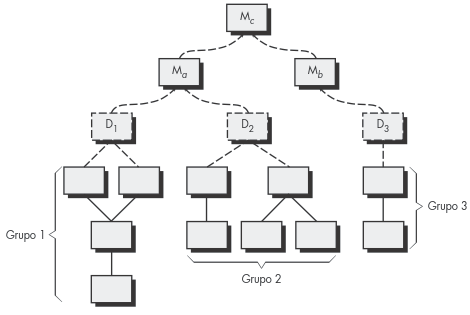
\includegraphics[scale=1]{project/images/integracion.png}
	\caption{\textbf{Integración Ascendente}}
\end{figure}
\subsubsection{Pruebas de regresión}
Cada vez que se agrega un nuevo módulo como parte de las pruebas de integración, el software cambia. Se establecen nuevas rutas de flujo de datos, ocurren nuevas operaciones de entrada o salida y se invoca una nueva lógica de control. Estos cambios pueden causar problemas con las funciones que anteriormente trabajaban sin fallas. En el contexto de una estrategia de pruebas de integración, las pruebas de regresión son la nueva ejecución de algún subconjunto de pruebas que ya se realizaron a fin de asegurar que los nuevos cambios no propagaron efectos no deseados.\\ En general, las pruebas exitosas, dan como resultado el descubrimiento de errores, los cuales son corregidos, cada vez que un error es corregido el software cambia. Las pruebas de regresión ayudan a garantizar que estos cambios no introducen comportamiento no planeado o errores adicionales.\\ Las pruebas de regresión se pueden realizar manualmente o usando herramientas de captura/reproducción, las cuales permiten capturar casos de prueba y resultados para una posterior reproducción y comparación. Las pruebas de regresión se extienden en tres clases diferentes de casos de prueba:
\begin{itemize}
	\item Una muestra representativa de prueba que evaluaran todas las funciones de software.
	\item Pruebas adicionales que se enfocan en las funciones del software que probablemente resulten afectadas por el cambio.
	\item Pruebas que se enfocan en los componentes del software que cambiaron.
\end{itemize}
Conforme avanzan las pruebas de integración, el número de pruebas de regresión puede volverse muy grande, por ende, es necesario que estas sean diseñadas para incluir a una o más clases de errores en cada una de las funciones del programa principal. Resulta impráctico e ineficiente volver a ejecutar todas las pruebas para cada función del programa cada que ocurre un cambio.
\subsubsection{Pruebas de humo}
La prueba de humo consiste en diseñar un mecanismo de ritmo para proyectos críticos en el tiempo, lo que le permite al equipo de software valorar el proyecto de manera frecuente. En general, las pruebas de humo abarcan las siguiente actividades:
\begin{enumerate}
	\item Los componentes se software se integran en una <<construcción>>, la cual incluye todos los archivos de datos, bibliotecas, módulos reutilizables y componentes necesarios que se requieren para implementar una o más funcionalidades del producto.
	\item Se diseña una serie de pruebas para exponer los errores que evitarán a la construcción realizar adecuadamente su función. Esto con la intención de encontrar los errores que puedan retrasar el proyecto.
	\item La construcción, una vez probada, se integra con otras construcciones y el producto (en su forma actual, considerando la cantidad de construcciones integradas) se prueba diariamente. Las construcciones se pueden integrar de manera ascendente o descendente.
\end{enumerate}
Algunas ventajas de implementar las pruebas de humo en un proyecto de software son:
\begin{itemize}
	\item Se minimiza el riesgo de implementación.
	\item La calidad del producto final mejora.
	\item La búsqueda y corrección de errores se simplifica.
	\item El progreso del proyecto es más fácil de valorar.
\end{itemize}
\subsubsection{Integración descendente vs Integración ascendente}
Como se ha analizado anteriormente, ambas estrategias de integración presentan sus respectivas ventajas y desventajas.\\
La selección de una estrategia de integración depende de las características del software y en ocasiones del calendario del proyecto. En general, un enfoque combinado puede resultar en el mejor arreglo.\\ Conforme se avanza en la integración, es necesario identificar los <<módulos críticos>>. Los cuales tienen al menos una de las siguientes características:
\begin{enumerate}
	\item Aborda muchos de los requerimientos del software.
	\item Tiene un alto nivel de control en la estructura del programa.
	\item Es complejo o propenso al error.
	\item Tiene requerimientos de rendimiento definidos.
\end{enumerate}
Estos módulos críticos deben de probarse tanto como sea posible.
\subsubsection{Productos de trabajo de las pruebas de integración}
Un plan global para integración del software y una descripción de las pruebas especificas se documentan en una <<Especificación de pruebas>>. Este producto de trabajo incorpora un plan de prueba y un procedimiento de prueba, y se vuelve parte de la configuración del software. Las pruebas de dividen en fases y construcciones que abordan características del software funcionales y de comportamiento específicas. Cada una de las fases de la prueba de integración delinea una amplia categoría funcional dentro del software y por lo general puede relacionarse con un dominio específico dentro de la arquitectura de software.\\ Los siguiente criterios y pruebas correspondientes se aplican a todas las fases de prueba:
\begin{itemize}
	\item Integridad de la interfaz: Las interfaces internas y externas se prueban conforme cada módulo (o grupo) se incorpora en la estructura.
	\item Validez funcional: Se realizan pruebas diseñadas para descubrir errores funcionales ocultos.
	\item Contenido de la información: Se realizan prueba diseñadas para descubrir errores ocultos asociados con las estructuras de datos locales o globales.
	\item Rendimiento: Se realizan pruebas diseñadas para verificar los limites del rendimiento establecidos durante el diseño de software.
\end{itemize}
En un <<Reporte de pruebas>>, que puede anexarse a la Especificación de pruebas, se registra una historia de resultados, problemas o peculiaridades de prueba reales. Como todos los demás elementos de una configuración de software, el formato de la especificación de pruebas puede adaptarse a las necesidades locales de la organización. Sin embargo, la estrategia de integración y los detalles de las pruebas son esenciales para cualquier especificación.
\subsection{Pruebas de Validación}
\paragraph{Verifican que el software cumpla con los requerimientos especificados.}
Después de la integración del software deben de evaluarse criterios de validación (establecidos durante el análisis de requerimientos).\\ Las pruebas de validación proporcionan la garantía final de que el software cumple con todos los requerimientos informativos, funcionales, de comportamiento y de rendimiento.\\ Se profundiza más en el tema en la sección \textbf{2.5}
\subsection{Pruebas del Sistema}
\paragraph{Verifican la funcionalidad total del sistema.}
El siguiente paso en las pruebas, consiste en que el software una vez validado, debe combinarse con otros elementos del sistema por ejemplo; Hardware, personal, bases de datos, etc.\\ Las pruebas de sistema verifican que todos los elementos se mezclan de una manera adecuada y que se logra el funcionamiento global del sistema.\\ Las pruebas de integración son una técnica sistemática para construir la arquitectura.\\ Se profundiza más en el tema en la sección \textbf{2.6}
\section{Estrategias de Prueba para Software Orientado a Objetos}
El objetivo de probar es encontrar el mayor número posible de errores con una cantidad manejable de esfuerzo aplicado durante un lapso de tiempo realista. A continuación se presentan algunas de las estrategias con las que puede ser probado el software orientado a objetos.
\subsection{Pruebas de unidad en el contexto Orientado a Objetos}
Cuando se considera software orientado a objetos, el concepto de unidad cambia. La encapsulación determina la definición de clases y objetos. Esto significa que cada clase y cada instancia de una clase empaqueta los atributos (datos) y las operaciones que manipulan estos datos.\\ En general, en una clase encapsulada es donde se realizan las pruebas de unidad. Sin embargo, los métodos de estas clases son las las unidades comprobables más pequeñas. Con esto, ya no es posible probar una sola operación en aislamiento sino más bien como parte de una clase.\\
La prueba de clase para software orientado a objetos es el equivalente de la prueba de unidad para software convencional. A las pruebas de clases la dirigen las operaciones encapsuladas por la clase y el comportamiento de estado de ésta.
\subsection{Pruebas de integración en el contexto Orientado a Objetos}
Debido a que como tal no existe una estructura de control jerárquico obvia entre las clases, las estrategias ascendente y descendente difícilmente pueden ser aplicadas. Pero, existen dos estrategias diferentes para realizar la integración.\\
La primera, es la llamada prueba basada en hebra, la cual integra el conjunto de clases requeridas para responder a una entrada o evento del sistema. Cada hebra se integra y prueba de manera individual. Las pruebas de regresión se aplica para asegurar que no ocurran efectos colaterales.\\ El segundo enfoque de integración, son las pruebas basadas en uso, comienzan con la construcción del sistema al probar las llamadas clases independientes. Después de probar las clases independientes, se prueba la siguiente capa de clases, llamadas dependientes, las cuales usan a las clases independientes. Esto se realiza de forma continua hasta que se integra todo el sistema.\\
El uso de controladores y representantes también cambian, los controladores pueden ser usados en un nivel más bajo y para la prueba de todos los grupos de clases, también pueden ser usados para sustituir una interfaz de usuario, de manera que la funcionalidad pueda ser probada antes de la implementación de la interfaz. Los representantes pueden usarse en situaciones donde se requiere la colaboración entre clases pero donde una o más de las clases colaboradoras todavía no se implementa por completo. 
\section{Estrategias de Prueba para Aplicaciones Web}
La estrategia para probar aplicaciones web adopta los principio básicos para todas las pruebas de software y aplica una estrategia y tácticas que se usan para sistemas orientados a objetos. En general puede resumirse en los siguientes pasos:
\begin{enumerate}
	\item El modelo contenido por la aplicación web se revisa para descubrir errores.
	\item El modelo de interfaz se revisa para garantizar que todos los casos de uso pueden adecuarse.
	\item El modelo de diseño para la aplicación web se revisa para descubrir errores de navegación.
	\item La interfaz de usuario se prueba para descubrir errores en los mecanismos de presentación y/o navegación.
	\item A cada componente funcional se le aplica una prueba de unidad.
	\item Se prueba la navegación a lo largo de toda la arquitectura.
	\item La aplicación web se implementa en varias configuraciones ambientales diferentes y se prueba su compatibilidad con cada configuración.
	\item Las pruebas de seguridad se realizan con la intención de explotar vulnerabilidades en la aplicación o en su ambiente.
	\item Se realizan pruebas de rendimiento.
	\item La aplicación se prueba mediante una población de usuarios finales controlada y monitoreada. Los resultados de su interacción con el sistema se evalúan por errores de contenido y de navegación, facilidad de uso, compatibilidad, confiabilidad y rendimiento.
\end{enumerate}
Puesto que muchas aplicaciones web evolucionan constantemente, el proceso de prueba es una actividad que se realiza siempre sobre la marcha, y se realiza para apoyar en las pruebas de regresión derivadas de las pruebas desarrolladas cuando se elaboro por primera vez aplicación web.
\section{Pruebas de Validación}
Las pruebas de validación comienzan en la culminación de las pruebas de integración, cuando ya han sido probados los componentes individuales y ya han sido completamente ensamblados como un paquete y los errores de interfaz se descubrieron y corrigieron. En las pruebas de validación desaparece la distinción entre software convencional, orientado a objetos u aplicaciones web. Las pruebas se enfocan en las acciones visibles para el usuario y las salidas del sistema reconocidas por el usuario.\\
Se pueden decir que la validación es exitosa cuando el software funciona en una forma que cumplas con las expectativas del cliente (lo especificado en el documento de requerimientos de software).
\subsection{Criterios de pruebas de validación}
La validación del software se logra mediante una serie de pruebas que demuestran conformidad con los requerimientos. Un plan de pruebas expresa las clases de pruebas que se van a realizar y un procedimiento de prueba define casos de prueba específicos que se diseñan para garantizar que se satisfagan todos los requerimientos.\\
Después de realizar cada caso de prueba de validación, existen dos posibles condiciones:
\begin{enumerate}
	\item La característica de función o rendimiento se conforma de acuerdo con las especificaciones y se acepta.
	\item Se descubre una desviación de la especificación y se crea una lista de deficiencias. Las cuales rara vez pueden ser corregidas antes de la entrega calendarizada.
\end{enumerate}
Además, es necesario que se tenga una descripción detallada de cada elemento que se desarrollo del software, esto para poder reforzar actividades de apoyo posteriores. A este proceso de revisión comúnmente se le conoce como <<Auditoría>>.
\subsection{Pruebas Alfa y Beta}
En la práctica, es complicado que un desarrollador de software prevea como usará el cliente final el programa. Algunas instrucciones pueden malinterpretarse, algunas salidas para el cliente podrían resultar poco claras para el. Cuando se construye software a la medida, se realizan una serie de pruebas de aceptación a fin de permitir al cliente validar todos los requerimientos. Estas pruebas son realizadas por el usuario final en lugar de un ingeniero de software.\\ Si el software se desarrolla como un producto que será usado por muchos clientes, no es práctico realizar este procedimiento, Para estos casos, son comúnmente usadas las pruebas alfa y beta.\\
\textbf{Las pruebas alfa} se llevan acabo en el sitio del desarrollador por un grupo representativo de usuarios finales El software se usa en el escenario natural con el desarrollador <<a un lado>> de los usuarios registrando errores y problemas de uso. Las pruebas alfa se realizan en un ambiente controlado.\\
\textbf{Las pruebas beta} se realizan en uno o más sitios del usuario final. Donde el desarrollador no se encuentra presente, por lo que las pruebas beta en realidad son la aplicación funcionando <<en vivo>> en un ambiente que no puede controlar el desarrollador. El cliente registra todos los problemas que se encuentre durante la prueba y los reporta al desarrollador periódicamente. Estos errores son corregidos y posteriormente el software vuelve a ser empaquetado y liberado para todos los clientes.
\section{Pruebas del Sistema}
El software, solo es un elemento de un sistema más grande, este debe de incorporarse con otros elementos del sistema, como hardware, personal, información. Para la cual se deben realizar las pruebas de sistema, las cuales son una serie de diferentes pruebas cuyo propósito principal es probar el sistema completo. Aunque cada prueba tenga un propósito diferente, todas funcionan para verificar que los elementos del sistema se hayan integrado de manera adecuada y que realicen las funciones asignadas.
En las siguientes secciones, se mencionan los tipos de prueba del sistema más importantes, como nota, las pruebas de sistema de carga y desempeño, se explican más detalladamente en secciones posteriores. 
\subsection{Pruebas de Recuperación}
La mayoría de los sistemas computacionales, deben de tener la capacidad de recuperarse de fallas y poder reanudar el procesamiento con poco o ningún tiempo de inactividad. A esto se le conoce, como un sistema tolerante a fallas, en los cuales, las fallas en el procesamiento no causan el cese de funcionamiento del sistema global.\\ La recuperación es una prueba del sistema que fuerza al software a fallar en varias formas y verifica que la recuperación se realice de manera adecuada. Si la recuperación es automática (el sistema la realiza en sí), se evalúa el reinicio, los mecanismos de puntos de verificación, la recuperación de datos y la reanudación para las correcciones. Si la recuperación requiere de intervención humana, se evalúa el tiempo medio de reparación para determinar si está dentro de los límites aceptables.
\subsection{Pruebas de Seguridad}
Cualquier sistema que gestione información sensible o cause acciones que puedan dañar (o beneficiar) de manera inadecuada a individuos puede ser blanco de intentos de penetración inadecuada o ilegal.\\
Las pruebas de seguridad, intentan verificar que los mecanismos de protección que se construyen en un sistema en realidad lo protegerán de cualquier intento de penetración ilegal. Durante estas, es necesario que se asuma el papel del individuo que intenta penetrar el sistema y es valido realizar probar con todo tipo de intentos. Por ejemplo, mediante el uso de software hecho a la medida para traspasar las defensas que se hayan construido, intentando abrumar el sistema para así negar el servicio a los demás usuarios, causando errores intencionalmente para intentar penetrar el sistema durante la recuperación, etc.\\ Las buenas pruebas de seguridad al final logran penetrar el sistema, pero se busca, que esta penetración resulte tan costosa (en tiempo y recursos) que sea de mayor valor que la información que se obtendrá del ataque en sí.
\subsection{Pruebas de Despliegue}
En determinados casos, el software debe ejecutarse en varias plataformas y bajo más de un entorno de sistema operativo. Las pruebas de despliegue, en ocasiones llamadas pruebas de configuración, prueban el software en cada entorno en el que este deba operar. Además, examina todos los procedimientos de instalación (esto incluye al software <<instalador>>) que usarán los clientes, así como toda la documentación que se usará para introducir el software a los usuarios finales.\\ En el caso de una aplicación web que funciona bajo el régimen de un navegador, es necesario probar la aplicación web en todos los navegadores sobre los que se piense dar soporte (comúnmente son todos los navegadores modernos) por lo cual aumenta la combinación de pruebas, ya que hay que probar cada navegador web sobre cada sistema operativos hasta cubrir todas las posibilidades (considerando que la compatibilidad entre los mismo lo permita). Las pruebas de seguridad están integradas en cada una de las pruebas de despliegue.